\section{Predator-Prey model}
This section describes the FLAMEGPU implementation of a simple predator-prey model. The specification of the model is based on the previous implementations on FLAME~\cite{Poulter} and NetLogo~\cite{netlogo}. We briefly give an introduction to the FLAMEGPU software in Section~\ref{sec:flamegpu} followed by details of the predator-prey model in Section~\ref{sec:preypredator}. Section~\ref{sec:implementation} gives an overview of the various components of the FLAMEGPU implementation.

\subsection{FLAMEGPU framwork}\label{sec:flamegpu}
FLAME GPU (a template driven framework for Agent Based Modeling on parallel architecture) is an extended version of the FLAME (Flexible Large-scale Agent-based Modelling Environment) framework~\cite{Coakley2016} that enables modellers from various disciplines like economics, biology and social sciences to easily write agent-based models, specifically for Graphics Processing Units (GPUs).

For a  more detailed and comprehensive overview of the framework followed by an example, please refer to our full tutorial paper to be published in HPCS17~\footnote{FLAME GPU: Complex System Simulation Framework}

\subsection{Problem description}\label{sec:preypredator}
To begin with, we give a very general description of the predator-prey model in the NetLogo library without reference to its implementation. Then we will give more details on the
implementation before describing the FLAMEGPU version in the next section.

The predator-prey model has 2 versions. In the more basic form, there are prey
and predators which preys move in a groups and try to avoid predators, while predators are moving towards preys and this costs a predator some energy. If, after a particular move, a predator and prey are close enough (within a fixed radius), the predator is able to eat the prey and increase the amount of energy it has. Predators die when they run out of energy.

The second version of the model includes grass (i.e. food source for preys) as an additional component. If preys move to a location which has grass, they are able to eat. This increases the amount of energy they have, but they can no longer move for free, as similarly to predators, with each move, some energy is lost. Preys will now die either when they are eaten by a predator, or if they run out of energy.

When a prey eats grass, the grass in that area is set to re-grow after a set length of time. Both
predators and preys are able to reproduce with a fixed probability rate at each time step.


The model has been implemented in various frameworks (e.g:NetLogo and FLAME). The implementation in FLAMEGPU is based on following details:


\begin{itemize}
\item Predator and Prey agents move and act in a sequence of iterations.
\item Predator and Prey agents have an (x, y) position and velocity.
\item Predator agents have an initial speed. Predator's speed increases when is close to a prey/group of preys.
\item A predator’s energy is reduced by 1 unit each time it moves.
\item Predator agents can only eat prey agents within a fixed radius.
\item A predator’s energy increases each time it catches a prey
\item A predator dies if it has run out of energy.
\end{itemize}
Additionally, when grass or preys' source of food is included in the model~\footnote{based on NetLogo's implementation}:
\begin{itemize}
%\item Each grass is either "green" or "navy", indicating whether grass is currently there.
\item A prey’s energy is reduced by 1 unit each time it moves.
\item A prey’s energy increases each time it eats grass.
\item A prey dies if it has run out of energy.
\item Once eaten, grass regrows after a fixed number of iterations.
\end{itemize}

The details of the algorithms at the decision points are given below.

\paragraph{Prey catching}
There is no limit on the amount of preys, a predator can eat per iteration. If there are multiple preys within the specific radius, predator can kill/eat them all. Moreover, a prey cannot be shared between multiple predators. If there are multiple predators and 1 prey within the killing distance, the first predator to attempt to catch the prey will do so.

\paragraph{Reproduction}
There is a set value for reproduction that can be different for predator and prey. At every iteration, we draw a random floating number between 0 to 1. If this number is less than the set value for reproduction then a new agent is created. The parent’s energy is shared with the new agent, so both will have half of the parent’s energy for the next iteration.

\subsection{FLAMEGPU implementation}\label{sec:implementation}
We designed the model based and implement the agent functions based on the assumption made in previous section. All agents have a position (x, y) in the domain as well as velocity. Moreover, predator agents also have an initial speed. In the basic model, only the predator agents have a variable (\verb|life|) which contains the amount of energy each have. However, in the second version of the model, in addition to the predators, prey agents also have a \verb|life| variable indicating the amount of energy they have.

In the case of implementing the second variant of the predator-prey model, grass agents have a boolean flag \verb|available| indicating whether there is currently grass at their location.

Moreover, unique ids are required for the predators and preys. When a predator kills a prey, it is necessary to know the id of both as this will be explained later in this section.

All communication between agents in FLAMEGPU is done via messages and in this model we have 3 messages ,or 5 when grass is included. The mechanism for "killing" is as follows:

\begin{enumerate}
\item Both prey and predator output their (x, y) coordinates to a location message.
\item Preys avoid predators
\item Predators read preys locations and move towards them
\item Prey read each others location and move towards each other producing flocking behaviour.
\item Predators read each others location and try to avoid each other by changing directions.
\item Prey reads locations of predators and if there was a predator in close enough proximity, then it outputs the \verb|prey_eaten_message| message and dies.
\item Predator read the \verb|prey_eaten_message| message and checks the id against its id. If the message indicates that the predator ate some prey, then increases its energy/life accordingly.
\end{enumerate}

When grass is included in the model a fourth and fifth message is required as a prey can only eat grass within a certain radius. The mechanism for "grazing" is as follows:

\begin{enumerate}
\item  Grass agents which currently have grass read the positions of the prey from the location
message.
\item  Grass agents read the positions of the prey from the location message. Then, each pick out the messages within the minimum distance and then post the ID of a prey within that distance to the \verb|grass_eaten_message| message. Note that if there is more than 1 prey on within the minimum distance, the grass agent will be eaten by the closest prey.
\item  Grass agents then modify the boolean flag to indicate they no longer have grass at this
time. The colour also changes from "green" to "navy".
\item  Prey agents read the \verb|grass_eaten_message| message which contain their ID. They then increase their energy accordingly.
\item Prey agents die if they dont' have enough life/energy
\end{enumerate}

\subsection{The FLAMEGPU Model}
Various elements of the FLAMEGPU model is as below:
\begin{itemize}
    \item \textbf{environment} - holds global information related to the simulation such as constant variables, C code file name
\item \textbf{agents} - all things related to the agents
\item \textbf{messages} - represent information which is communicated between agents
\end{itemize}

To download the predator-prey \verb|XMLModelFile.xml|, follow the instructions given in Section~\ref{sec:hands-on}. Various tags have been used to define the model. Please refer to the FLAMEGPU user manual for detail~\cite{richmond11b}.
\subsubsection{FLAMEGPU environment}
The environment section contains various user defined constants and specific functions. For the Predator-Prey model, some of the parameters that define the behaviour of the agents are included in the environment section. 
\begin{verbatim}
<gpu:environment>
    <gpu:constants>
        <gpu:variable>
            <type>float</type>
            <name>REPRODUCE_PREY_PROB</name>
            <defaultValue>0.03</defaultValue>
        </gpu:variable>
        <gpu:variable>
            <type>float</type>
            <name>REPRODUCE_PREDATOR_PROB</name>
            <defaultValue>0.03</defaultValue>
        </gpu:variable> 
        <gpu:variable>
            <type>int</type>
            <name>GAIN_FROM_FOOD_PREDATOR</name>
            <defaultValue>15</defaultValue>
        </gpu:variable>
        <gpu:variable>
            <type>int</type>
            <name>GAIN_FROM_FOOD_PREY</name>
            <defaultValue>5</defaultValue>
        </gpu:variable>
    </gpu:constants>
    <gpu:functionFiles>
        <file>functions.c</file>
    </gpu:functionFiles>
    <gpu:initFunctions>
        <gpu:initFunction>
            <gpu:name>initLogFile</gpu:name>
        </gpu:initFunction>
    </gpu:initFunctions
    <gpu:exitFunctions>
        <gpu:exitFunction>
            <gpu:name>closeLogFile</gpu:name>
        </gpu:exitFunction>
    </gpu:exitFunctions>
    <gpu:stepFunctions>
        <gpu:stepFunction>
            <gpu:name>outputToLogFile</gpu:name>
        </gpu:stepFunction>
    </gpu:stepFunctions>
</gpu:environment>
\end{verbatim}
\subsubsection{Agent memory}
The agent definition is tagged by \verb|<xagents>|. Agent memory variables are defined in this section. Below is an examples of "grass" agent memory containing multiple agent variables:

\begin{verbatim}
<memory>
    <gpu:variable>
        <type>int</type>
        <name>id</name>
    </gpu:variable>
    <gpu:variable>
        <type>float</type>
        <name>x</name>
    </gpu:variable>
    <gpu:variable>
        <type>float</type>
        <name>y</name>
    </gpu:variable>
    <gpu:variable>
        <type>float</type>
        <name>type</name>
    </gpu:variable>
    <gpu:variable>
        <type>int</type>
        <name>level</name>            
    </gpu:variable>
    <gpu:variable>
        <type>int</type>
        <name>available</name>            
    </gpu:variable>
</memory> 
\end{verbatim}



\subsubsection{Agent functions} % Func description from Paul's Tutorial @ Rabat
The Functions aspect of the agent description describes the properties of the behaviours that the agent will have. Note: This is not where the actual behaviour is described but the properties relating to the behaviour functions. Table~\ref{tab:1} and Table~\ref{tab:2}, shows the list of defined functions per agent in the predator-prey model. 


\begin{table}[h]
\centering
\caption{Summary of the Prey agent functions for Predator Prey model - no grass included}
\begin{tabular}{ |l|l| } 
\hline
Function & Description\\
\hline\hline
prey\_output\_location& each prey agent outputs information to be read by other agents\\\hline
prey\_avoid\_pred& prey agents avoiding predator agents\\\hline
prey\_flock& flocking between prey agents\\\hline
prey\_move & movement of prey agents\\\hline
prey\_eaten & prey agents get killed by predator agents\\\hline
prey\_eat\_or\_starve & prey agents gain energy or starve (only when grass included in the model)\\\hline
prey\_reproduction & regeneration of preys\\
\hline
\end{tabular}
\label{tab:1}
\end{table}

\begin{table}[h]
\centering
\caption{Summary of the Predator agent functions for Predator Prey model - no grass included}
\begin{tabular}{ |l|l| } 
\hline
Function & Description\\
\hline\hline
pred\_output\_location& each predator agent outputs information to be read by other agents\\\hline
pred\_follow\_prey& predator agents follow prey agents\\\hline
pred\_avoid& predator agents avoid each other\\\hline
pred\_move & movement of predator agents\\\hline
pred\_eat\_or\_starve & predator agents gain energy or starve\\\hline
prey\_reproduction & regeneration of predators\\
\hline
\end{tabular}
\label{tab:2}
\end{table}



Functions are applied to agents in a specified initial\_state and will result in the agent moving into a next\_state (or the same state). Furthermore, functions can have conditions. For example, a function which simulates agent death might check a variable incremented each iteration called life-cycles to see if it has reached a maximum number. Only agents meeting this condition would perform the behaviour and move into a dead state.  The predator-prey model is a fairly simple model and does not have any function conditions.

Functions can have either a single input or output (or neither). Inputs and outputs are in the form of messages which are a collection of variables which are persistent from the point in which they are output to the end of the simulation iteration (at which point they are destroyed).  A function description within a model requires that any inputs or outputs are fully specified. 



Listing~\ref{lst:XML_output_func} shows the structure of a Function description in a model. In this example, the agent function has a message output which updates the agents internal memory. In order to add a new agent function, simply add the the XML code to the model after the existing function definitions.


\begin{lstlisting}[linewidth=\columnwidth,breaklines=true,language=C++,caption={},label=lst:XML_output_func]
<gpu:function>
    <name>prey_output_location</name>
    <currentState>default1</currentState>
    <nextState>default1</nextState>
    <outputs>
        <gpu:output>
            <messageName>prey_location</messageName>
            <gpu:type>single_message</gpu:type>
        </gpu:output>
    </outputs>
    <gpu:reallocate>false</gpu:reallocate>
    <gpu:RNG>false</gpu:RNG>
</gpu:function>
\end{lstlisting}

The additional reallocate and \verb|RNG| tags are used to specify if the agent function may result in agent death (reallocate) or if a random number generator is required (RNG). 

Note that for each message type defined within the XMML model definition, the dynamically generated simulation API will create a message output function. Agents can only output a single message per agent function. In Listing~\ref{lst:output_func}, agent prey outputs a message with three variables.

\begin{lstlisting}[linewidth=\columnwidth,breaklines=true,language=C++,caption={},label=lst:output_func]
__FLAME_GPU_FUNC__ int pred_output_location(xmachine_memory_predator* xmemory, xmachine_message_pred_location_list* pred_location_messages)
{
	add_pred_location_message(pred_location_messages, xmemory->id, xmemory->x, xmemory->y);
	return 0;
}
\end{lstlisting}

Moreover, iterating over message input (message list) within agent function is also possible by the use of dynamically generated message API functions. Listing~\ref{lst:eaten_func} shows a complete agent function with input messages demonstrating the iteration of a message list and outputting a different message. The while loop (\verb|while (pred_location_message)|) continues until the \verb|get_next_pred_location_message| return a NULL or a false value. 


\begin{lstlisting}[linewidth=\columnwidth,breaklines=true,language=C++,caption={},label=lst:eaten_func]
__FLAME_GPU_FUNC__ int prey_eaten(xmachine_memory_prey* xmemory, xmachine_message_pred_location_list* pred_location_messages, xmachine_message_prey_eaten_list* prey_eaten_messages)
{
	int eaten = 0;
	int predator_id = -1;
	float closest_pred = PRED_KILL_DISTANCE;

	//Iterate the predator location messages until NULL is returned which indicates all messages have been read.
	xmachine_message_pred_location* pred_location_message = get_first_pred_location_message(pred_location_messages);
    while (pred_location_message)
	{
		//calculate distance between prey and predator
		float2 predator_pos = float2(pred_location_message->x, pred_location_message->y);
		float2 prey_pos = float2(xmemory->x, xmemory->y);
		float distance = length(predator_pos - prey_pos);

		//if distance is closer than nearest predator so far then select this predator as the one which will eat the prey
		if (distance < closest_pred)
		{
			predator_id = pred_location_message->id;
			closest_pred = distance;
			eaten = 1;
		}

		pred_location_message = get_next_pred_location_message(pred_location_message, pred_location_messages);
	}

	//if one or more predators were within killing distance then notify the nearest predator that it has eaten this prey via a prey eaten message.
	if (eaten)
		add_prey_eaten_message(prey_eaten_messages, predator_id);

	//return eaten value to remove dead (eaten == 1) agents from the simulation
	return eaten;
}
\end{lstlisting}


After adding the function definition to the XML model file, the new function should be added to the layers. Layers represent synchronisation points in the execution of the agent functions. It is assumed that functions on the same layer execute simultaneously so functions which have a dependency via messages should not be within the same layer. The \verb|prey_output_location|, \verb|prey_follow_prey| and \verb|prey_flock| functions are in different layers for this reason. 

In the case of \verb|prey_output_location| function, it will be added to the layer so that it executes in the same layer as \verb|pred_output_location|. The other functions are are added after the output location function to ensure they begins executing after all prey agents have completed outputting each prey's location (Listing~\ref{lst:XML_layer}).

\begin{lstlisting}[linewidth=\columnwidth,breaklines=true,language=C++,caption={},label=lst:XML_layer]
<layer>
    <gpu:layerFunction>
        <name>prey_output_location</name>
    </gpu:layerFunction>
    <gpu:layerFunction>
        <name>pred_output_location</name>
    </gpu:layerFunction>
</layer>
<layer>
    <gpu:layerFunction>
        <name>prey_flock</name>
	</gpu:layerFunction>
	<gpu:layerFunction>
        <name>pred_avoid</name>
	</gpu:layerFunction>
</layer>
<layer>
...
</layer>
\end{lstlisting}



\subsubsection{Agent messages}
All the agent communication is done via messages. In the second version of the model with grass included, we have five different message types: \textit{predator\_location}, \textit{prey\_location},\textit{grass\_location}, \textit{prey\_eaten}, \textit{grass\_eaten}. These messages contain all the required information by other agents in order to interact with each other. The description of \verb|grass_location| message is as below:
\begin{verbatim}
<messages>
    <gpu:message>
        <name>grass_location</name>
        <description>a message holding the location of an agent</description>
        <variables>
            <gpu:variable>
               <type>int</type>
               <name>id</name>
            </gpu:variable>
            <gpu:variable>
               <type>float</type>
               <name>x</name>
            </gpu:variable>
            <gpu:variable>
               <type>float</type>
               <name>y</name>
            </gpu:variable>
        </variables>
        <gpu:partitioningNone/>
        <gpu:bufferSize>262144</gpu:bufferSize>
    </gpu:message>
..
<messages>
\end{verbatim}

To download the complete XML model file for both versions of the model, follow the instructions given in Section~\ref{sec:hands-on}.

\subsection{The FLAMEGPU flow diagram}
Figure~\ref{fig:flowdiagram1} and Figure~\ref{fig:flowdiagram2} shows the dependency graph for the Predator-Prey model with and without grass implementation.

\begin{figure}[h]
    \centering
    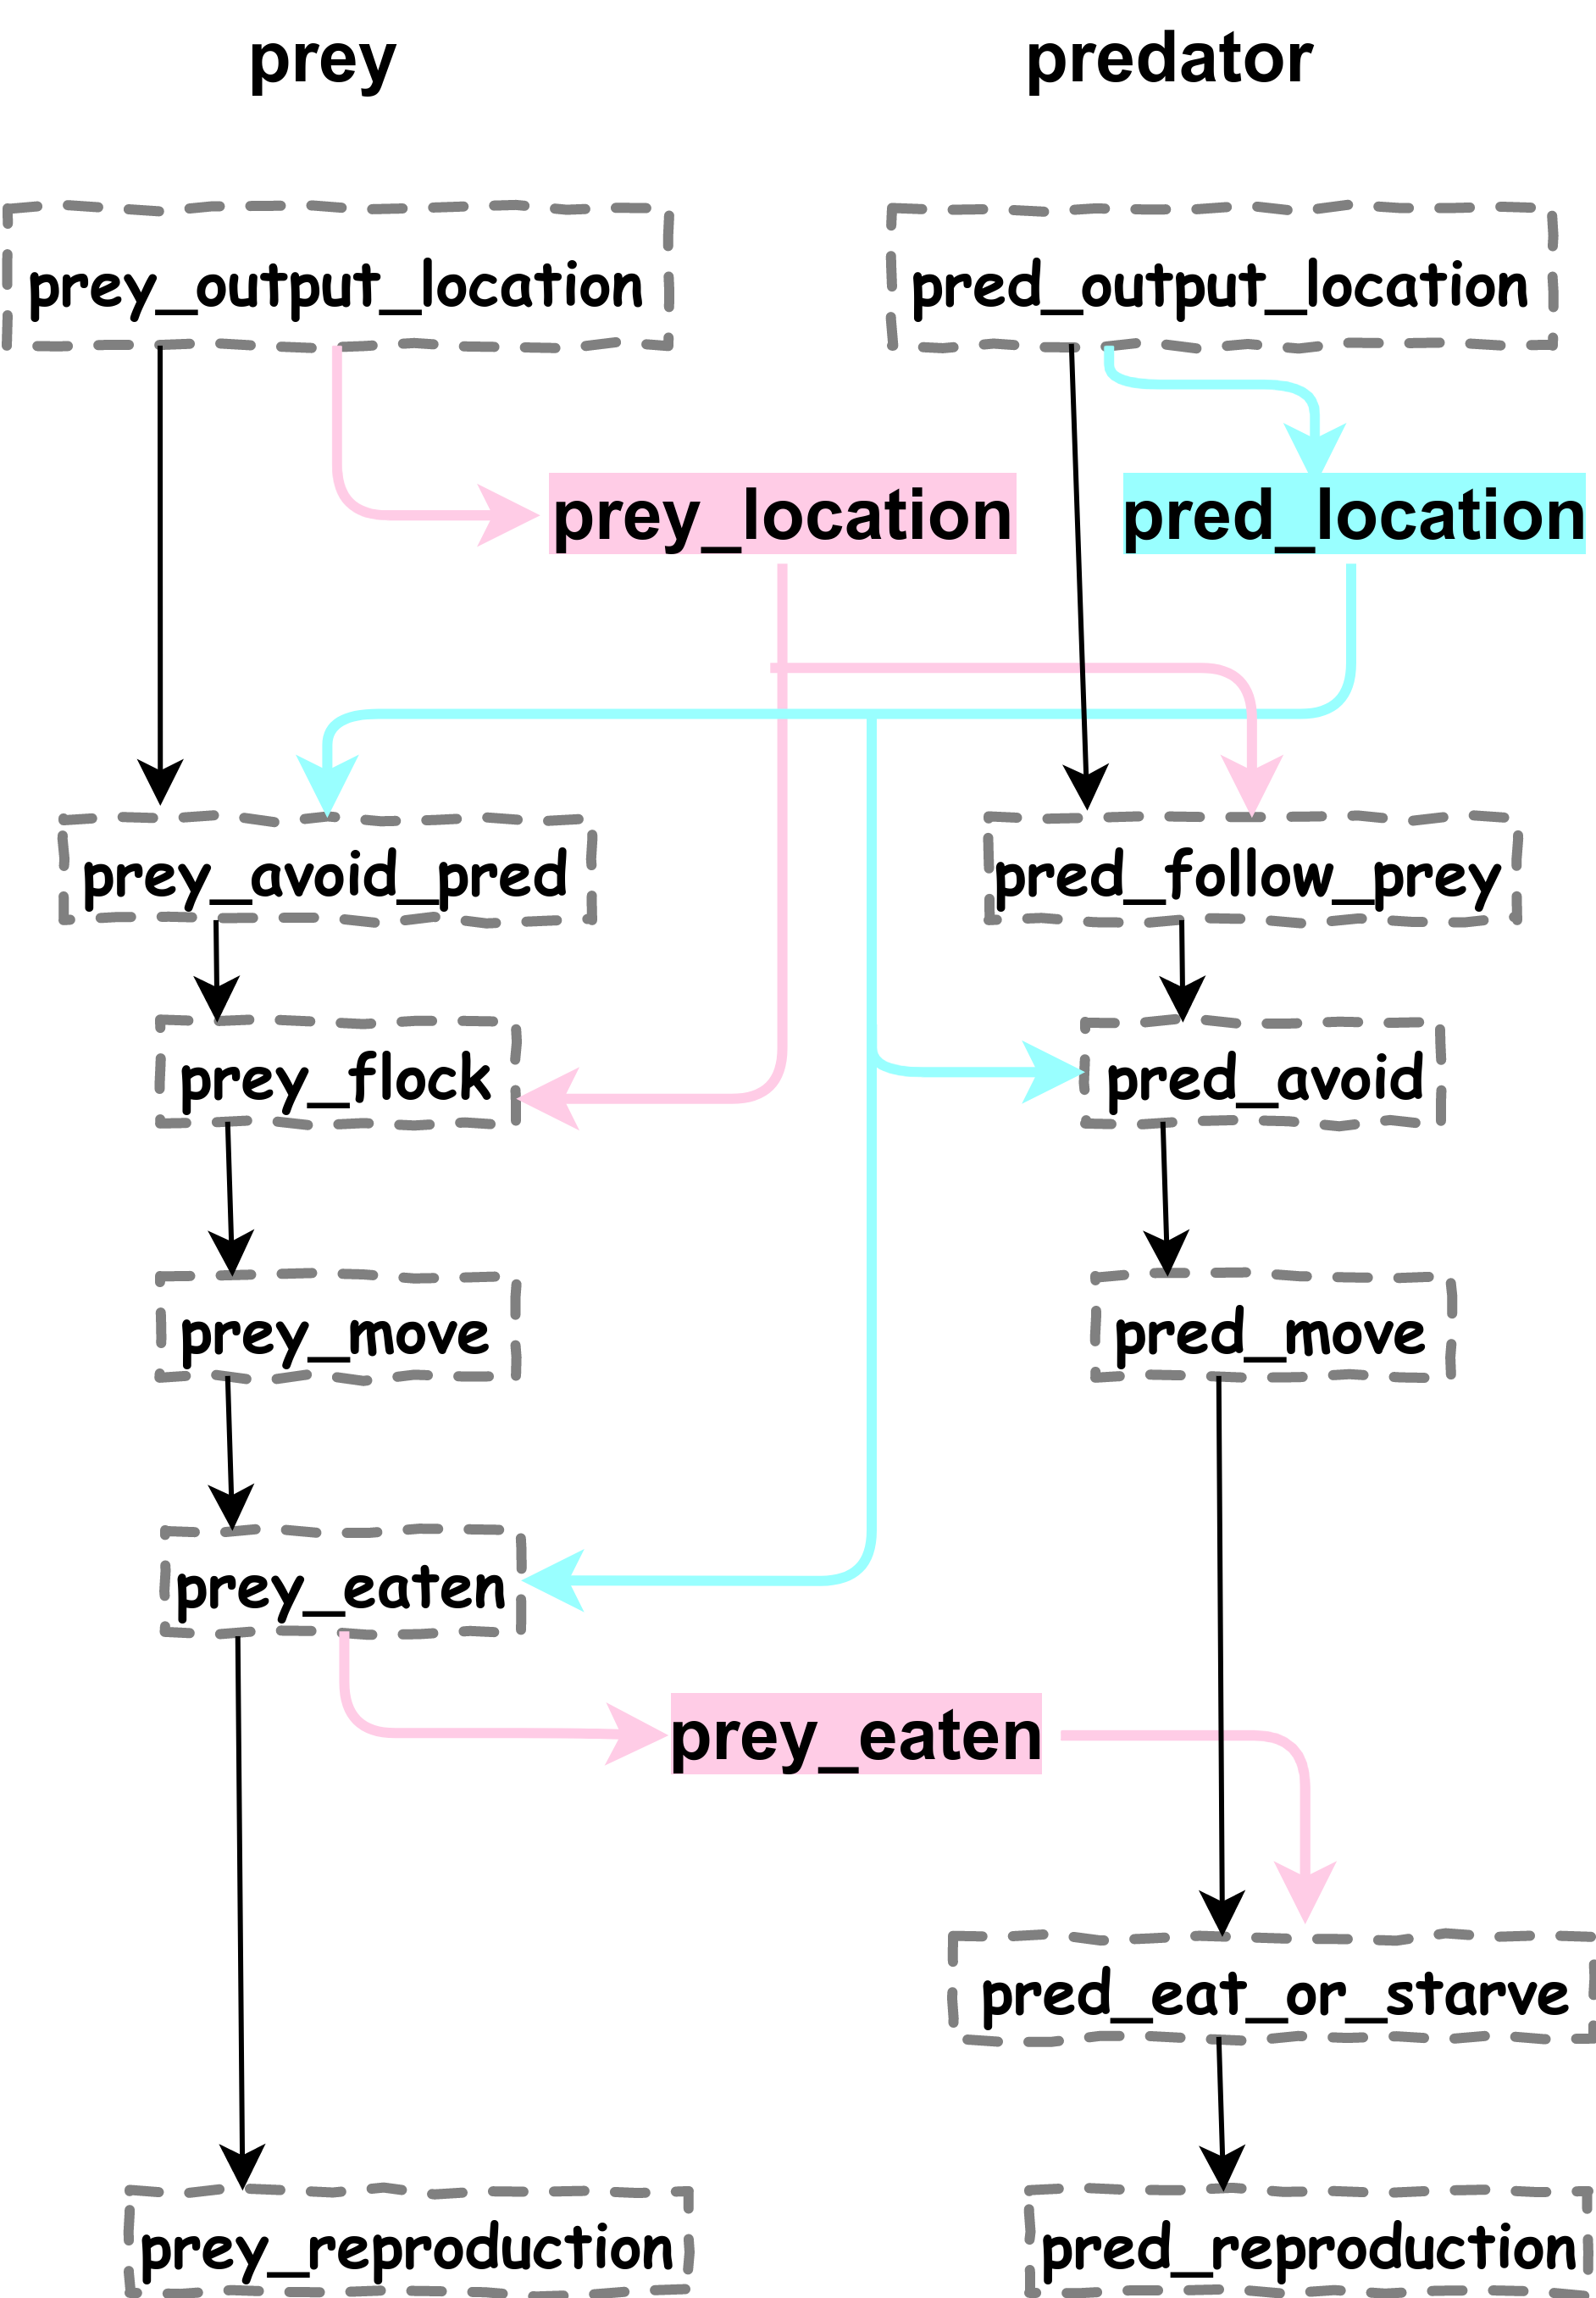
\includegraphics[width=3.2in]{prey_pred}
    \caption{Flow diagram for Predator-Prey model without grass}
    \label{fig:flowdiagram1}
\end{figure}

\begin{figure}[h]
    \centering
    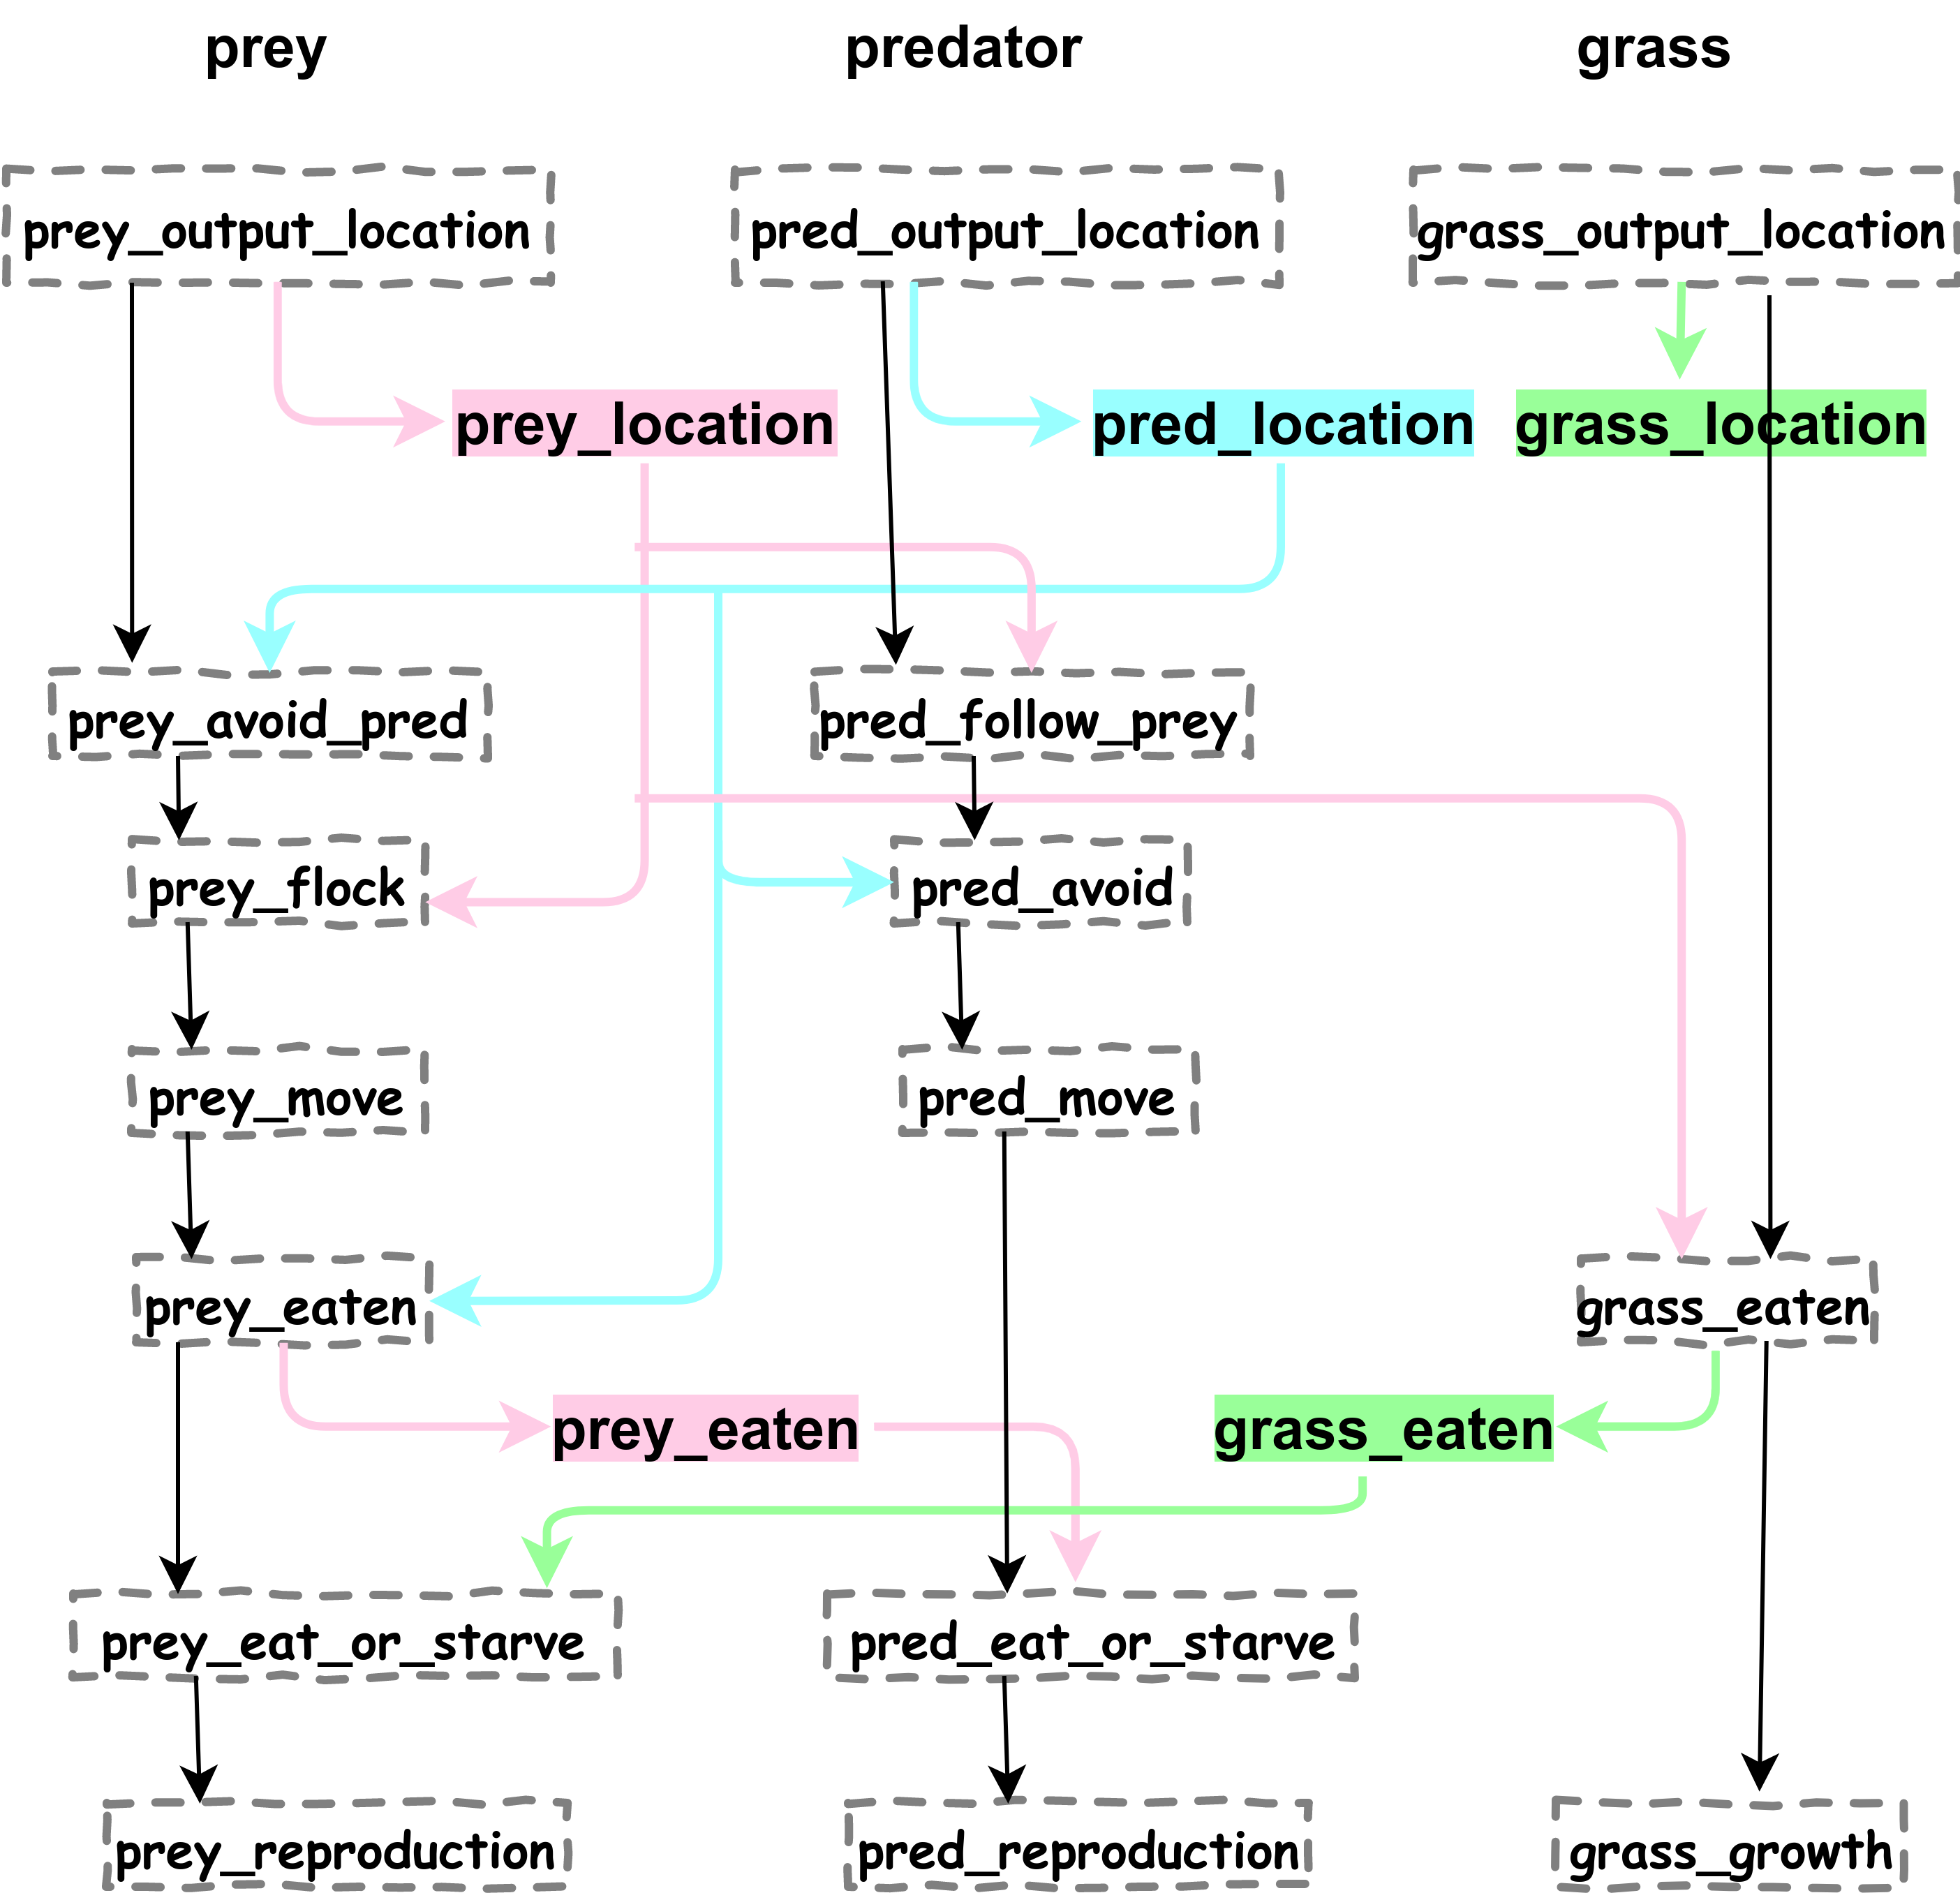
\includegraphics[width=4.2in]{prey_pred_grass}
    \caption{Flow diagram for Predator-Prey model with grass}
    \label{fig:flowdiagram2}
\end{figure}

\clearpage
\subsection{Input data generation and Setup}
The initial data for the model is generated using a simple c++ program. The program generates the specified number of predator and prey agents in random positions (\verb|x,y|) between [-1,1] with random velocities (\verb|fx,fy|) between [-1,1]. Moreover, each predator is given an amount of energy (\verb|life|) which is randomly selected from the interval of [0,40]. This interval is chosen to align the initial data close to the FLAME and NetLogo implementation. 

In the case where grass in included, prey agents require an energy (\verb|life|) variable similar to predators. This variable is randomly selected from the interval of [0,50]. The grass agent initial colour is set to "green". Once eaten, the \verb|available| variable is set to 0 and it takes upto \verb|GRASS_REGROW_CYCLES| iterations till the grass re-grow. 

The program generates an \verb|0.xml| output file containing the initial data. Table~\ref{tab:param} shows the various parameters used for the implementation of the model in FLAMEGPU.

\begin{table}[h]
\centering
\caption{Summary of parameters in Predator Prey model - grass included}
\begin{tabular}{ |l|l| } 
\hline
Parameter & Value \\
\hline\hline
Initial number of prey agents & 800\\\hline
Initial number of predator agents & 400\\\hline
Initial number of grass agents & 2000\\\hline
Amount of energy gained from eating prey & 75\\\hline
Amount of energy gained from eating grass & 50\\\hline
Probability of predators reproducing & 0.03\\\hline
Probability of preys reproducing & 0.05\\\hline
Number of iterations before grass can re-grow & 100\\
\hline
\end{tabular}
\label{tab:param}
\end{table}

